\documentclass[11pt,a4paper]{article}

\usepackage[T1]{fontenc}
\usepackage[utf8]{inputenc}
\usepackage{lmodern}
\usepackage[margin=2.3cm]{geometry}
\usepackage{graphicx}
\usepackage{booktabs}
\usepackage{amsmath,amssymb}
\usepackage{siunitx}
\usepackage{xcolor}
\usepackage{caption}
\usepackage[hidelinks]{hyperref}
\usepackage[capitalise,noabbrev]{cleveref}

\sisetup{detect-all}
\newcommand{\code}[1]{\texttt{\detokenize{#1}}}
\newcommand{\pos}{\textcolor{green!45!black}{$\blacktriangle$}}
\newcommand{\negv}{\textcolor{red!70!black}{$\blacktriangledown$}}
\newcommand{\neu}{\textcolor{gray}{$\bullet$}}

\title{Predicting Unit Commitment in Short-Term Hydropower Scheduling\\[2pt]
\large TDT4173 Modern Machine Learning in Practice --- Course Project}
\author{Team \textit{[team name]}: Stefano Videsott, \textit{[member 2]}, \textit{[member 3]}}
\date{\today}

\begin{document}
\maketitle

\begin{abstract}
We predict, for each of the 14 generating units of the Tokke--Vinje hydropower system and each hour of a
one-week scheduling horizon, the probability that the unit is committed (on) in the solution of the SHOP
optimiser. Our final model is a blend of four LightGBM and two XGBoost models trained on a long-format table
with one row per (case, unit, hour) and 157--224 engineered features. The decisive features encode the plant
economics: the hourly price relative to the water value of the reservoir feeding the unit, and the length of
the contiguous period during which that ratio stays above one, a proxy for start-up and shut-down costs.
A second step came from reading the topology more carefully: several plants draw from a tiny head pond that is
fed by, or tunnel-connected to, a much larger lake, and describing the storage of that \emph{effective}
reservoir group added another $+0.0006$. With a time-blocked, purged cross-validation the blend reaches a
micro ROC-AUC of 0.9853 out of fold and 0.99126 on the public Kaggle leaderboard. We also report the ideas
that did \emph{not} work (sequence neural networks, stacking across units and cases, a separate week-level
model, pseudo-labelling, using future reservoir volumes) and why.
\end{abstract}

%=====================================================================
\section{Problem and evaluation}
%=====================================================================
Short-term hydropower scheduling decides, hour by hour, how much each unit produces. The binary on/off
\emph{unit commitment} (UC) variables make the underlying mixed-integer programme expensive to solve; a good
prediction of them can be used to fix or relax binaries and speed up the optimisation.

Each \emph{case} is a 168-hour week starting at midnight UTC; a new case starts every day, so consecutive
cases overlap by six days. The training set has 2\,922 cases (2015-01-01 to 2022-12-31) and the test set
725 cases (2023-01-01 to 2024-12-25). For every case we must output $14 \times 168 = 2\,352$ probabilities.
The score is the \emph{micro-averaged} ROC-AUC: all $725 \times 2\,352 \approx 1.7$ million predictions are
pooled into a single ranking. Two consequences guided the work:
\begin{itemize}
  \item predictions must be comparable \emph{across units and weeks}, not only within one unit's week;
  \item knowing which units are on (or off) for an entire week already gives a large share of the score.
\end{itemize}
The public leaderboard covers 2023 and the private one 2024, so the public score is only an estimate.

%=====================================================================
\section{Data and exploratory analysis}
%=====================================================================
\paragraph{Inputs.} Hourly day-ahead price (EUR/MWh) and inflow to 17 reservoirs and one river; daily
storage volume and water value (EUR/MWh) of the 17 reservoirs; hourly minimum-volume (3 reservoirs) and
minimum-flow (6 rivers) constraints; and the SHOP topology file with reservoir capacities, generator limits,
turbine curves and the connections between objects. We turned the raw tables into per-case arrays
(\code{src/data.py}): price $168$, inflow $18\times168$, volume and water value $17\times8$ (days $0..7$,
day $7$ being the end of the horizon), constraints, and labels $14\times168$. There are no missing values.

\paragraph{Topology.} From the connection list we derived, for each plant, the reservoir(s) it draws from and
the reservoir it releases into (\cref{tab:topo}). This mapping is the backbone of the feature engineering.
The immediate intake is not always where the water is stored. Haukeli's intake Vatjern holds only
0.3\,Mm$^3$ and is fed by the river from Langeidvatn (32\,Mm$^3$); Vaamarvatn (Vinje) is joined to Totak
(258\,Mm$^3$) and Foersvatn (Kjela) to Bordalsvatn by tunnels with equal start and end height, so their levels
move together; Kjelavatn (Vesle Kjela) is fed by Staavatn. We call the intake plus these lakes the
\emph{effective upstream storage} of a plant (last column of \cref{tab:topo}).

\begin{table}[ht]
\centering\footnotesize
\caption{Plants, units and their reservoirs (from \code{Tokke_Vinje_topology.yaml}). $q_{\max}$ is the largest
turbine discharge on the efficiency curves. Last column: effective upstream storage used by the
\code{--topo2} features.}
\label{tab:topo}
\setlength{\tabcolsep}{3pt}
\begin{tabular}{lcllrrl}
\toprule
Plant & Units & Intake & Releases into & $P_{\max}$ & $q_{\max}$ & Effective upstream storage\\
 & & & & [MW] & [m$^3$/s] & \\
\midrule
Tokke       & 4 & Vinjevatn              & Bandak      & 107.5 & 32    & Vinjevatn, Totak, Vaamarv., Venemo\\
Vinje       & 3 & Vaamarvatn             & Vinjevatn   & 100   & 55    & Totak, Vaamarvatn\\
Songa       & 1 & Songavatn, Bitdalsvatn & Totak       & 120   & 52    & (same)\\
Kjela       & 1 & Foersvatn              & Hyljelihyl  & 60    & 40    & Foersvatn, Bordalsvatn\\
Lio         & 1 & Byrtevatn              & river       & 43    & 14    & (same)\\
Byrte       & 1 & Botnedalsvatn          & Byrtevatn   & 20    & 8     & (same)\\
Hogga       & 1 & Bandak                 & --          & 17    & 168.6 & (same)\\
Vesle Kjela & 1 & Kjelavatn              & Foersvatn   & 8.5   & 20    & Kjelavatn, Staavatn\\
Haukeli     & 1 & Vatjern                & Vinjevatn   & 4.9   & 2.1   & Langeidvatn, Vatjern\\
\bottomrule
\end{tabular}
\end{table}

\paragraph{Label structure.} About half of the (case, unit) pairs are constant for the whole week
(\cref{fig:eda}); in mixed weeks a unit switches only 2--6 times, i.e.\ decisions come in long blocks.
Base rates differ strongly (Vinje G3 is on 26\% of the hours, Lio 75\%).

\begin{figure}[ht]
\centering
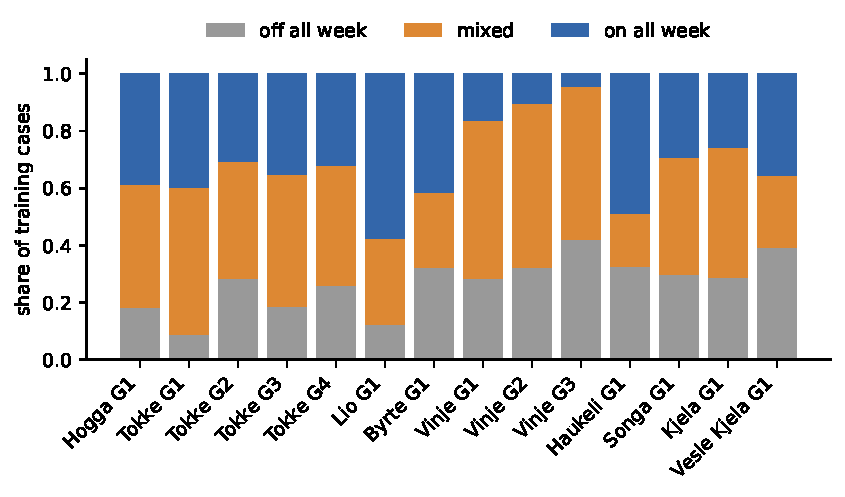
\includegraphics[width=.8\linewidth]{figures/eda_units.pdf}
\caption{Weekly behaviour per unit on the training cases: share of weeks where the unit is off all week, on
all week, or switches.}
\label{fig:eda}
\end{figure}

\paragraph{Label noise.} Hour $t+24$ of case $d$ and hour $t$ of case $d+1$ refer to the same wall-clock hour,
yet they agree only 88\% of the time. The optimum depends on the horizon end (end-of-week water values), so
the same hour is scheduled differently from one case to the next. Any model that ignores the case context
is bounded by this.

\paragraph{Simple baselines.} On the training set a per-unit constant (the unit's base rate) gives
0.617 AUC, the within-week price rank 0.589, and price minus the water-value difference 0.539. The
relationship is clearly non-linear and unit-specific.

\paragraph{Economic intuition.} \Cref{fig:examples} (left) shows the typical pattern: a Tokke unit runs when the
price exceeds the water value of its upstream reservoir and stops during short, deep price dips. The right
panel shows the hard case: with an almost flat price the decision is driven by water balance (Tokke releases
into Bandak, so Hogga must eventually run) and the model misses it.

\begin{figure}[ht]
\centering
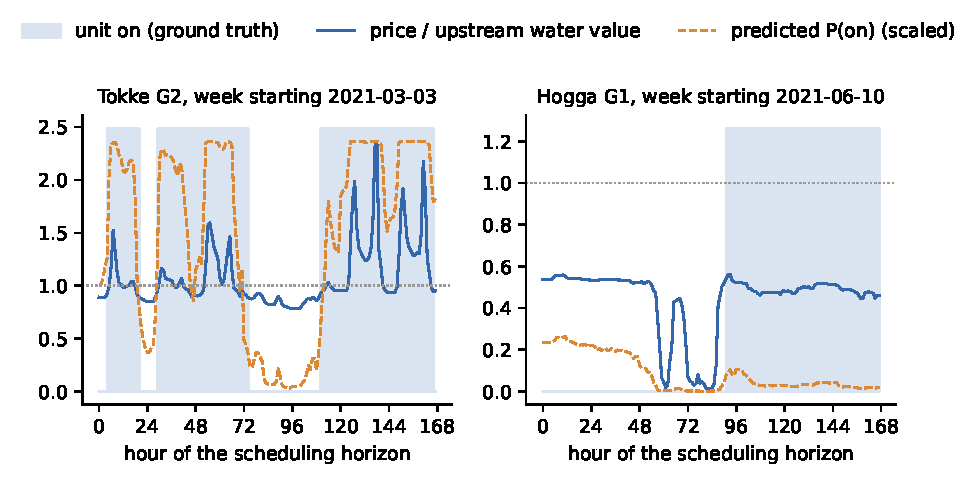
\includegraphics[width=\linewidth]{figures/example_weeks.pdf}
\caption{Two training weeks. Shaded: ground-truth commitment. Solid: price divided by the end-of-horizon water
value of the upstream reservoir (dotted line at 1). Dashed: out-of-fold prediction of the final blend.}
\label{fig:examples}
\end{figure}

%=====================================================================
\section{Validation strategy}
%=====================================================================
Random K-fold would leak: a case and its neighbours share six of their seven days. We used four
\emph{time-blocked} folds of two years each (2015--16, 2017--18, 2019--20, 2021--22) and removed from
training every case starting within 7 days of the validation block (purge). All numbers in this report
are out-of-fold (OOF) micro ROC-AUC on the 2\,922 training cases unless stated otherwise. For quick
experiments we trained on a 20\% row subsample with a higher learning rate and evaluated only folds 2--3
(2019--22); repeating such a run with another seed moved the scores by about $\pm0.0005$, which sets the
threshold for calling an idea an improvement.

The repeated runs of the final setting showed that a single fold can move by up to $\pm0.001$ with the
row subsample alone, so we only adopted changes that improved several folds at once. The CV turned out to be
a reliable guide: over seven submissions every OOF gain reappeared on the public leaderboard with about the
same size (\cref{fig:progress}), from \code{gbm_v2} (0.9826 / 0.98881) to the final blend (0.9853 / 0.99126).

%=====================================================================
\section{Feature engineering}
%=====================================================================
The model works on a long table with one row per (case, unit, hour): $3\,647 \times 14 \times 168 \approx
8.6$ million rows (\code{src/features.py}). Features are grouped as follows (the version in which each group
was introduced is given in brackets).

\begin{description}
  \item[Price shape (v1).] Raw price, z-score and ratio to the weekly mean, rank within the week and within the
  day, deviation from the daily mean, centred rolling means (3--25\,h), differences to the previous/next hour,
  weekly quantiles; later (v2) mean of the next and previous 24\,h.
  \item[Calendar (v1).] Hour of horizon, hour of day, day of week, month and day-of-year (sin/cos).
  \item[Reservoir state (v1--v2).] For all 17 reservoirs: initial filling ratio, end-of-horizon and initial
  water value (absolute and relative to the mean price); mean inflow per reservoir; constraint series.
  \item[Unit static (v1).] Unit id (categorical), $P_{\min}$, $P_{\max}$, start cost, generator index within
  the plant, number of generators in the plant.
  \item[Plant economics (v1--v3).] With $w^{\uparrow}$ the end-of-horizon water value of the upstream
  reservoir(s) and $w^{\downarrow}$ that of the downstream one: the price minus, and divided by,
  the difference $w^{\uparrow}-w^{\downarrow}$;
  \textbf{price over $w^{\uparrow}$} (\code{p_over_upwv}), the share of hours whose ratio exceeds
  $\{0.8, 0.9, 1, 1.1, 1.25\}$, and \code{rank_m_need_up} = price rank minus the rank threshold implied by that
  share (positive when the hour is among the hours worth producing in).
  \item[Run lengths (v3).] Start-up and shut-down costs make it unprofitable to react to short spikes or dips.
  For the boolean series ``ratio $>1$'' we compute the signed length of the run containing hour $t$
  (\code{seg_up_len}), the position inside it and the hours left; the same for ``price $>$ water-value
  difference''.
  \item[Water balance (v4/v5).] Filling of the upstream and downstream reservoir if the unit does not release
  (initial volume plus cumulative natural inflow, optionally plus the maximal discharge of the plants feeding
  it), hours until full, hours to empty the reservoir at full discharge, room left downstream.
  \item[Cross-plant (v4, v7, v9).] Every plant's price/water-value ratio and run length at hour $t$, visible to
  every unit, to let e.g.\ Hogga see what Tokke is likely to do.
  \item[Effective upstream storage (v6--v9, \code{--topo2}).] For the reservoir group of \cref{tab:topo}:
  initial filling, capacity-weighted end-of-horizon water value (relative to the mean price and to the intake's
  water value), weekly inflow relative to capacity, hours until full, filling trajectory without release, and
  price over the group's water value with its share above one and run length.
  \item[Effective downstream storage (v7, v8, \code{--dn2}).] The same for the lakes the discharge ends up in
  (e.g.\ Hyljelihyl and Venemo for Kjela, Vinjevatn and Bandak for Vinje), plus price against the water-value
  difference between the two groups. It did not improve a single model but adds diversity to the blend.
\end{description}

\paragraph{Future volumes were deliberately excluded.} The volume table also contains the storage on days
$1..7$ of each horizon, which is available for the test period. Adding the weekly volume change lowered the
2021--22 fold from 0.9695 to 0.9653. The daily release implied by these volumes correlates weakly
($|r|\le0.24$) with the daily on-hours, so the volumes describe the historical operation of the system, not
the SHOP solution we predict, and they act as noise.

%=====================================================================
\section{Models}
%=====================================================================
\paragraph{Gradient boosting (final).} LightGBM~\cite{lightgbm} with binary log-loss, 255 leaves, at least 200
rows per leaf, feature fraction 0.5, bagging 0.7, $L_2=10$, learning rate 0.05, early stopping on the
validation fold (150 rounds), 30--40\% row subsampling to fit in 30\,GB of RAM. The test model is refit on all
training cases with $1.1\times$ the mean best iteration. A single model trains in 15--25 minutes on 8 CPU cores.
We ran half of the full trainings in parallel on an Azure ML cluster (one 16-vCPU F16s\_v2 node, student
subscription, scaled to zero when idle).

\paragraph{XGBoost.} The same table and the same hyper-parameters translated to XGBoost~\cite{xgboost}
(histogram method, loss-guided growth with 255 leaves, \code{min_child_weight} 20) scored higher than
LightGBM on identical features (0.9827 vs.\ 0.9821 on 2019--22) and stops after two to three times as many
trees. The two XGBoost models together get 40\% of the final blend weight.

\paragraph{Ensemble.} Logit averages of models that differ in library, feature set and seed. With more than
five candidates the grid search on the simplex becomes too slow, so we used greedy ensemble selection
(20 steps, with replacement) on the OOF predictions. The final weights are
v2 0.30, v7 0.15, v8 0.10, v9 0.05, XGB v1 0.15, XGB v2 0.25; equal weights over the same models give 0.9851.

\paragraph{Neural networks (not used in the final submission).} (i) A transformer over the 168 hours of a case
with static context and a $14\times168$ output head, from raw inputs: 0.914 on 2021--22.
(ii) A dilated temporal convolutional network over the GBM feature table, one sequence per (case, unit),
receptive field above 168\,h: 0.957 on 2021--22, with a training loss far below the validation loss. Both
overfit the 2\,922 weeks. In a blend with the GBM they add at most $+0.0008$, and without a GPU (none was
available in our quota) each fold took about 20 minutes, which ruled out further tuning.

%=====================================================================
\section{Results}\label{sec:results}
%=====================================================================

\begin{table}[ht]
\centering\small
\caption{Full four-fold results. Scores are micro ROC-AUC; Kaggle = public leaderboard (2023).}
\label{tab:main}
\setlength{\tabcolsep}{4pt}
\begin{tabular}{lrrrrrrr}
\toprule
Model & \#feat. & 2015--16 & 2017--18 & 2019--20 & 2021--22 & OOF & Kaggle\\
\midrule
GBM v1 (price + reservoirs)           & 136 & 0.9813 & 0.9799 & 0.9546 & 0.9695 & 0.9716 & --\\
GBM v2 (+ plant economics)            & 157 & 0.9861 & 0.9840 & 0.9745 & 0.9850 & 0.9826 & 0.98881\\
GBM v3 (+ run lengths)                & 172 & 0.9863 & 0.9836 & 0.9750 & 0.9863 & 0.9833 & --\\
GBM v4 (+ water bal., cross-plant)    & 207 & 0.9874 & 0.9842 & 0.9702 & 0.9875 & 0.9830 & --\\
GBM v5 (+ water balance)              & 180 & 0.9871 & 0.9843 & 0.9745 & 0.9860 & 0.9835 & --\\
GBM v6 (v5 + eff.\ upstream)          & 189 & 0.9879 & 0.9846 & 0.9751 & 0.9867 & 0.9841 & --\\
GBM v7 (v4 + eff.\ up-/downstream)    & 224 & 0.9883 & 0.9849 & 0.9730 & 0.9879 & 0.9841 & --\\
GBM v8 (v5 + eff.\ up-/downstream)    & 197 & 0.9876 & 0.9844 & 0.9759 & 0.9873 & 0.9842 & --\\
GBM v9 (v4 + eff.\ upstream, lr 0.03) & 216 & 0.9882 & 0.9852 & 0.9734 & 0.9883 & 0.9842 & --\\
XGB v1 (features of v6)               & 189 & 0.9884 & 0.9851 & 0.9775 & 0.9871 & 0.9842 & --\\
XGB v2 (features of v7)               & 224 & 0.9884 & 0.9854 & 0.9761 & 0.9879 & 0.9845 & --\\
\midrule
Blend v2 + v4                         &     & 0.9873 & 0.9846 & 0.9757 & 0.9871 & 0.9842 & 0.99045\\
Blend v2 + v3 + v4 + v5               &     & 0.9873 & 0.9847 & 0.9763 & 0.9870 & 0.9844 & 0.99043\\
Blend v2 + v4 + v6                    &     & 0.9879 & 0.9849 & 0.9768 & 0.9873 & 0.9848 & 0.99084\\
Blend v2 + v6 + v7 + v8               &     & 0.9882 & 0.9851 & 0.9770 & 0.9879 & 0.9851 & 0.99109\\
Blend v2 + v7 + v8 + v9 + XGB v1      &     & 0.9884 & 0.9854 & 0.9778 & 0.9880 & 0.9853 & 0.99117\\
\textbf{Final:} above + XGB v2         &     & 0.9885 & 0.9855 & 0.9781 & 0.9880 & \textbf{0.9853} & \textbf{0.99126}\\
\bottomrule
\end{tabular}
\end{table}

\begin{figure}[ht]
\centering
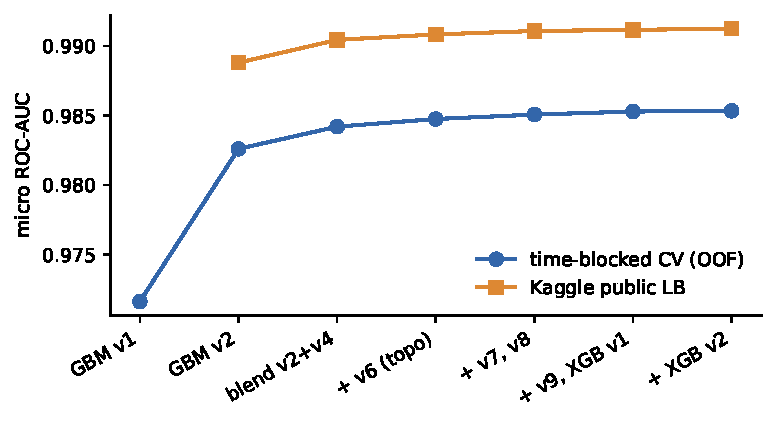
\includegraphics[width=.55\linewidth]{figures/progress.pdf}
\caption{Out-of-fold CV and public leaderboard. Improvements in CV carried over to the leaderboard one-to-one.}
\label{fig:progress}
\end{figure}

\paragraph{Ablations and negative results.} \Cref{tab:ablation} lists every experiment we evaluated, including
those that did not help. Most ideas that should help in principle (more context, more coupling between units,
post-processing) did not beat the noise level of $\pm0.0005$.

\begin{table}[ht]
\centering\small
\caption{Experiments on folds 2019--20 / 2021--22 (quick setting) or on the full OOF. \pos\ adopted,
\neu\ neutral, \negv\ rejected.}
\label{tab:ablation}
\begin{tabular}{p{6.6cm}p{5.9cm}c}
\toprule
Idea & Result & \\
\midrule
Future weekly volume change & 2021--22: 0.9695 $\to$ 0.9653 & \negv\\
Plant economics (price / water value, need rank) & 2019--20: 0.9546 $\to$ 0.9736; 2021--22: 0.9695 $\to$ 0.9845 & \pos\\
Run lengths above threshold & 0.9736 / 0.9845 $\to$ 0.9744 / 0.9856 & \pos\\
Cross-plant features & 0.9744 / 0.9856 $\to$ 0.9707 / 0.9864 & \neu\ (diversity)\\
Water balance & 0.9744 / 0.9856 $\to$ 0.9741 / 0.9853 & \neu\ (diversity)\\
Lags/leads and windowed max/min of the ratio & $\to$ 0.9738 / 0.9848 & \negv\\
Stronger regularisation (63 leaves, 2000 rows/leaf) & $\to$ 0.9748 / 0.9848 & \neu\\
Stacking with neighbouring cases' predictions (same hour) & every fold below its base model & \negv\\
Stacking with all units' predictions & OOF 0.9718 vs.\ 0.9826 base & \negv\\
Temporal smoothing of the logits & best 0.98436 vs.\ 0.98437 & \negv\\
Per-unit logit recalibration & 0.9837 vs.\ 0.9844 & \negv\\
Pseudo-labelling the unlabeled period & matches its teacher; $+0.00005$ in blend & \neu\\
Transformer / TCN sequence models & 0.914 / 0.957 alone; $\le+0.0008$ in blend & \negv\\
Ensembling GBMs with different feature sets & OOF 0.9835 (best single) $\to$ 0.9844; Kaggle $+0.0016$ & \pos\\
\midrule
\multicolumn{3}{l}{\emph{Second round (full-quality setting, compared with v5 on the same seed)}}\\
Lower learning rate (0.05 $\to$ 0.02) & 0.9810 $\to$ 0.9813 alone; $\pm0$ in blend & \neu\\
Twice as many training rows (30\% $\to$ 60\%) & 0.9810 $\to$ 0.9809 & \negv\\
Effective upstream storage (\code{--topo2}) & 0.9745 / 0.9860 $\to$ 0.9764 / 0.9868; full OOF 0.9835 $\to$ 0.9841 & \pos\\
Effective downstream storage (\code{--dn2}) & 0.9821 $\to$ 0.9816 alone; useful in blend & \neu\ (diversity)\\
XGBoost instead of LightGBM & 0.9821 $\to$ 0.9827; +0.0002 in blend & \pos\\
Average with the overlapping cases (same wall-clock hour) & 0.9844 $\to$ 0.9836 at weight 0.2, worse above & \negv\\
Week-level model re-levelling the hourly logits & 0.9844 $\to$ 0.9843 at weight 0.1, worse above & \negv\\
\bottomrule
\end{tabular}
\end{table}

\paragraph{Error analysis.} \Cref{fig:breakdown} breaks the OOF score down. The weakest units are Vinje G3
(the third unit, started only when G1 and G2 are not enough), Haukeli (4.9\,MW) and Hogga (driven by the water
Tokke releases into Bandak). Haukeli gained most from the effective-storage features (0.9605 $\to$ 0.9667):
its intake Vatjern is too small to store anything, and what matters is how full Langeidvatn is. 2020, a year
with exceptionally low prices and high inflow, is clearly the hardest.

\emph{Where is the remaining error?} If we shift each (case, unit) row of the blend's logits so that its mean
probability equals the true share of on-hours in that week, and keep the predicted order of the hours, the
OOF AUC rises from 0.9844 to 0.9971. Almost all of the remaining error is therefore in \emph{how much} a unit
runs in a week, not \emph{when}. The mean absolute error of the predicted weekly share is 0.065, and it is
largest for weeks in which the unit runs 25--75\% of the time (0.14). A dedicated week-level model
(one row per case and unit, 434 weekly aggregates) predicted the share worse (0.079) than the hourly blend,
and mixing it in did not help (\cref{tab:ablation}).

\begin{figure}[ht]
\centering
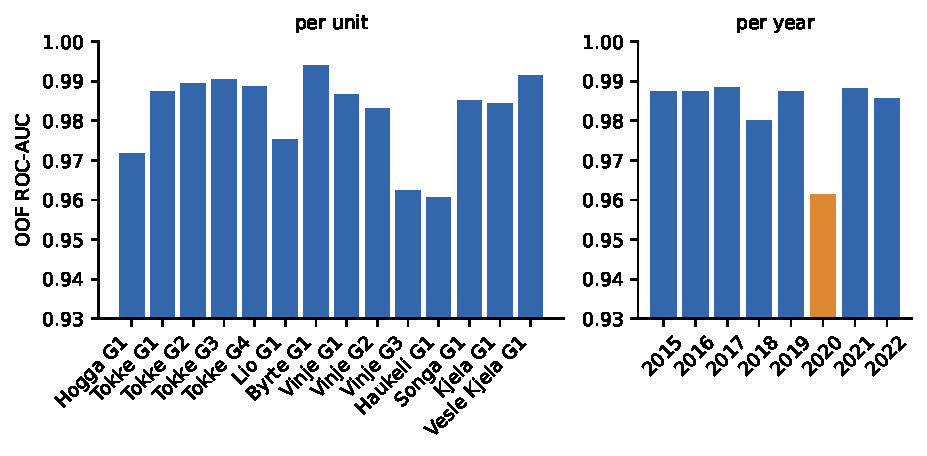
\includegraphics[width=.95\linewidth]{figures/auc_breakdown.pdf}
\caption{Out-of-fold AUC of the final blend per unit and per year.}
\label{fig:breakdown}
\end{figure}

\paragraph{Model interpretation.} \Cref{fig:importance} shows the split-gain importance. The model is dominated
by the run length \code{seg_up_len} and \code{p_over_upwv}, followed by the unit identity, Tokke's price
ratio (a cross-plant feature) and the ``need rank''. Physically this means: a unit runs when power is worth more
than the water it uses, and only if that holds long enough to pay for starting it. The water value of the
effective upstream storage (\code{up2_wv7rel}, \code{up2_p_over_wv}) comes right after, ahead of the water
value of the small Vinjevatn reservoir where Tokke, Vinje and Haukeli meet.

\begin{figure}[ht]
\centering
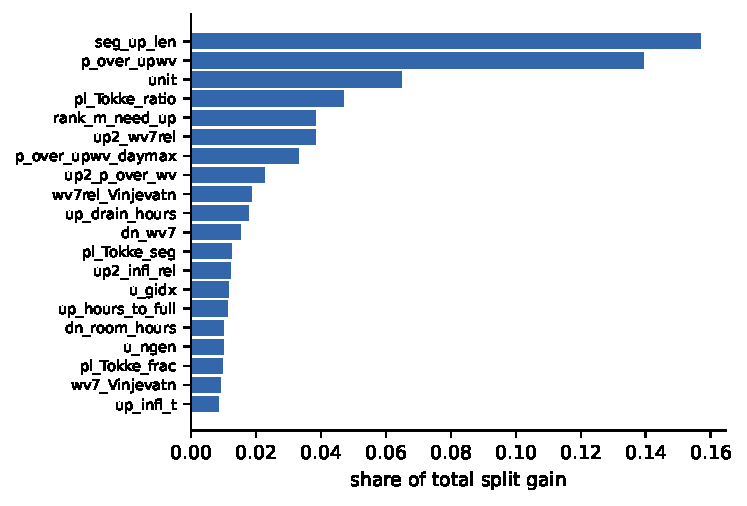
\includegraphics[width=.55\linewidth]{figures/importance.pdf}
\caption{Top-20 features by LightGBM split gain (v9 feature set: cross-plant and effective upstream storage;
model trained on 2015--20).}
\label{fig:importance}
\end{figure}

%=====================================================================
\section{Discussion and limitations}
%=====================================================================
\begin{itemize}
  \item \textbf{Independence assumption.} Every (unit, hour) is predicted on its own. Units are coupled through
  the watercourse, and our attempts to model this (stacking, cross-plant features, joint neural networks) either
  overfit or did not transfer across years. A joint sequence model trained on a GPU is the most promising
  direction we could not explore properly.
  \item \textbf{Weekly level.} The order of the hours within a week is almost solved; the open problem is the
  number of hours each unit runs (\cref{sec:results}). That number follows from the water budget of the whole
  watercourse over the horizon, which per-hour features describe only approximately.
  \item \textbf{Distribution shift.} Year-to-year scores range from 0.965 (2020) to 0.989; the private
  leaderboard (2024) may therefore differ from the public one.
  \item \textbf{Irreducible variability.} Overlapping cases agree only 88\% on the same hour. Part of the
  remaining error is due to the optimiser's sensitivity to the horizon end and to near-equivalent MIP solutions.
\end{itemize}

%=====================================================================
\section{Conclusion}
%=====================================================================
Feature engineering grounded in the physics and economics of the watercourse was what moved the score:
expressing the price relative to the water value of the reservoir that feeds each unit (0.9716 $\to$ 0.9826)
and adding the length of the profitable period (0.9833). Describing the storage that each plant really draws
from, instead of its immediate intake, gave the best single LightGBM model (0.9841). A blend of LightGBM and
XGBoost models with different feature sets gave the final 0.9853 OOF / 0.99126 public AUC. Tuning
(learning rate, more rows, more regularisation) and post-processing did not help. A purged, time-blocked
validation was essential: it predicted the leaderboard gains and let us reject many attractive but useless
ideas.

\paragraph{Reproducibility.} All code is in \code{src/}; see \cref{app:repro}.

\begin{thebibliography}{9}
\bibitem{lightgbm} G.~Ke et al., ``LightGBM: A highly efficient gradient boosting decision tree,'' in
\emph{Advances in Neural Information Processing Systems 30}, 2017.
\bibitem{xgboost} T.~Chen and C.~Guestrin, ``XGBoost: A scalable tree boosting system,'' in \emph{Proc.\ 22nd ACM
SIGKDD}, 2016.
\bibitem{shop} SINTEF Energy Research, \emph{SHOP --- Short-term Hydro Operation Planning, documentation},
\url{https://docs.shop.sintef.energy}.
\end{thebibliography}

\appendix
\section{Reproducing the results}\label{app:repro}
\begin{footnotesize}
\begin{verbatim}
uv venv --python 3.12 .venv
uv pip install --python .venv pandas numpy scikit-learn lightgbm \
    xgboost pyyaml pyarrow matplotlib
.venv/bin/python src/data.py               # build cache/cases.npz
# gbm_v2 was trained before later feature groups were added (commit b3d90c8)
T=".venv/bin/python src/train_gbm.py --sub 0.3 --no-future-vol --full"
$T --name gbm_v7 --topo2 --dn2 --seed 4
$T --name gbm_v8 --topo2 --dn2 --no-cross --seed 7
$T --name gbm_v9 --topo2 --lr 0.03 --rounds 5000 --seed 9
$T --name xgb_v1 --algo xgb --topo2 --no-cross --seed 5
$T --name xgb_v2 --algo xgb --topo2 --dn2 --seed 11
.venv/bin/python src/blend.py --greedy gbm_v2 gbm_v7 gbm_v8 \
    gbm_v9 xgb_v1 xgb_v2                    # weights on OOF
.venv/bin/python src/submit.py gbm_v2:0.3 gbm_v7:0.15 gbm_v8:0.1 \
    gbm_v9:0.05 xgb_v1:0.15 xgb_v2:0.25 --out submissions/blend_final.csv
.venv/bin/python report/make_figures.py    # figures of this report
# Azure ML: az ml job create -f azure/v7_job.yml (same for v9, xgb2)
\end{verbatim}
\end{footnotesize}

\end{document}
